\capitulo{6}{Aspectos relevantes del desarrollo del proyecto}

Este punto contiene, de manera descriptiva y detallada, el proceso seguido desde el inicio hasta el fin del proyecto. 

Cómo ya se ha comentado en el punto anterior de la memoria, la metodología utilizada ha sido CRISP-DM, y es por ello que el orden de este punto se debe a las diferentes fases. A continuación, se describe detalladamente cada una de las 6 fases.

\section{Entendimiento del negocio}
En esta primera fase se ha buscado información sobre el proceso de galvanizado, con el fin de ponerse en contexto con el tema del proyecto y entender a que se dedica la empresa que da origen a este trabajo. 

A continuación, se puso en contexto el objetivo principal del proyecto, que es, sobre unos datos tomados por sensores en la cadena de producción, crear un modelo capaz de predecir si una bobina podrá ser aprovechable por parte de la empresa o no, en función de si el recubrimiento de zinc cumple unos estándares.

Los sensores toman datos de cada una de las \emph{tejas} de la bobina. Una \emph{teja} es una porción de bobina, de entre unos 10 y 25 metros (según el tipo de sensor), sobre la que se mide la capa de zinc para posteriormente almacenar su valor.

Además, cada bobina tendrá una cantidad de zinc mínimo y máximo estipulado que tendrá que cumplir para que pueda ser utilizada en el escenario para la que se está construyendo. 

\section{Entendimiento de los datos}
La empresa nos ha proporcionado datos que han sido tomados en la cadena de producción, y que han sido evaluados previamente por un operario, otorgándoles dos posibles clases:
\begin{itemize}
    \item \textbf{OK:} la bobina es válida y puede ser usada por la empresa. 
    \item \textbf{NOK:} la bobina no cumple con los requisitos del cliente y/o la empresa y, por tanto, será descartada.
\end{itemize}

Cabe destacar que una bobina, a pesar de que tenga alguna \emph{teja} que incumpla los requisitos de zinc, puede ser aprovechable por la empresa. Por ejemplo, la Figura \ref{f:visu} muestra los diferentes valores de zinc medidos en una bobina por cada sensor, junto con las líneas verdes entre las que se debería de encontrar la capa zinc. En dichas gráficas se pueden ver claramente como hay varias \emph{tejas} que incumplen los requisitos (puntos que no se encuentran entre las dos líneas verdes). Pese a todo, la clase otorgada a esta bobina por parte del operario es OK.

\subsubsection{Tipos de datos}
En primer lugar, hay que conocer los tipos de datos proporcionados, ya que según los sensores que los miden (se explicarán más adelante), los datos tomados de la bobina pueden ser 1D o 2D:
\begin{itemize}
    \item \textbf{Datos 1D:} los datos se van tomando \emph{teja} por \emph{teja}, de forma que realmente se está construyendo un vector unidimensional. La Figura \ref{f:datos1D} lo muestra mucho más claro de forma gráfica, donde, en primer lugar, se miden los datos de la \emph{teja} 1, a continuación los de la \emph{teja} 2 y así sucesivamente hasta leer toda la bobina.
    \begin{figure}[h]
     \centering
      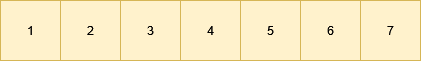
\includegraphics[width=0.9\textwidth]{img/1D.png}
     \caption{Ejemplo estructura datos 1D}
     \label{f:datos1D}
    \end{figure}
    \item \textbf{Datos 2D:} en este otro tipo de datos, en vez de utilizar un único sensor, se usan 9, de forma que sobre cada \emph{teja} se toman 9 datos diferentes. La Figura \ref{f:datos2D} muestra como sería el proceso de lectura de datos. En primer lugar, se lee la primera \emph{teja} y sobre ella se toman 9 valores (celdas 1 a la 9), a continuación se toman datos de la \emph{teja} 2 y se toman otros 9 datos (celdas 10 a 18). En definitiva, sobre cada bobina se está construyendo una matriz de 9 filas y un número de columnas cambiante en cada caso, según como de larga sea la bobina.
    \begin{figure}[h]
     \centering
      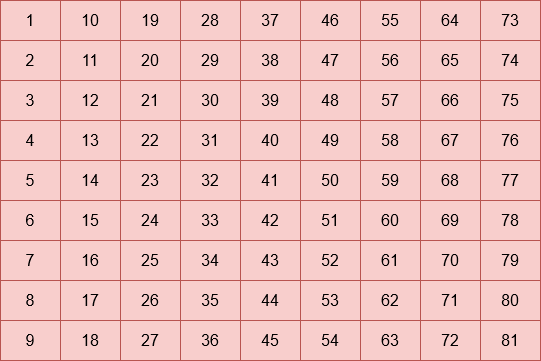
\includegraphics[width=0.9\textwidth]{img/2D.png}
     \caption{Ejemplo estructura datos 2D}
     \label{f:datos2D}
    \end{figure}
    \end{itemize}

\subsubsection{Tipos de sensores}
Antes de empezar a explicar que atributo tiene cada tipo de dato, es importante conocer cómo funcionan los diferentes sensores, ya que cada uno de ellos opera de una forma diferente para medir los datos. En total existen 6 sensores diferentes, cada uno de ellos nombrado con una ID diferente:
\begin{itemize}
    \item \textbf{123:} se corresponde con un sensor de datos 1D que mide la capa superior de la bobina. Toma datos cada 25 metros.
    \item \textbf{124:} se corresponde con la pareja del sensor 123, pero toma datos de la capa inferior de la bobina.
    \item \textbf{201:} se corresponde con otro sensor de datos 1D, pero diferente al anteriormente mencionado, de la capa superior. Este sensor también toma datos cada 25 metros.
    \item \textbf{202:} es la pareja del sensor 201. Toma medidas de la capa inferior de la bobina.
    \item \textbf{1234:} es un sensor de los datos 2D y toma datos de la capa superior de la bobina. Los datos son tomados cada 10 metros.
    \item \textbf{1243:} es la pareja del sensor 1234, y toma datos de la capa inferior de la bobina.
\end{itemize}

\subsubsection{Datos proporcionados}
Los datos proporcionados se encuentran en una base de datos MySQL, y divididos en tres tablas. A continuación se recoge el nombre de cada una de ellas, junto con los principales atributos que serán utilizados en el proyecto:
\begin{itemize}
    \item \textbf{GR\_LPValues:} contiene un total de 115972 registros de los datos 1D. Cada registro se corresponde para una bobina, sensor y \emph{teja} específica. Los principales atributos son:
    \begin{itemize}
        \item \textbf{COILID:} se corresponde con la ID de la bobina.
        \item \textbf{TILEID:} se corresponde con la ID de la \emph{teja} de la bobina. Cada \emph{teja} tiene diferente ID, su orden es cronológico, es decir, la primera \emph{teja} será el valor más pequeño, la segunda \emph{teja}, el segundo valor más pequeño, y así sucesivamente.
        \item \textbf{MID:} se corresponde con la ID del sensor que ha capturado los datos. Estos valores son los mencionados anteriormente, dónde se explicaba como funcionaba cada sensor.
        \item \textbf{MEAN:} contiene el valor medio de zinc en dicha teja. Este es el valor utilizado para ver si cumple o no con los requisitos de zinc.  
        \end{itemize}
    Un ejemplo de los diferentes atributos que componen esta tabla se pueden ver en la Figura \ref{f:tab1}.
    \begin{figure}[h]
     \centering
      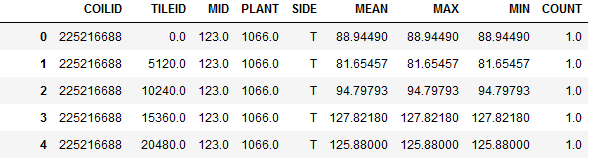
\includegraphics[width=0.9\textwidth]{img/eje1D.PNG}
     \caption{Ejemplo tabla GR\_LPValues}
     \label{f:tab1}
    \end{figure}
    \item  \textbf{GR\_QPValues:} contiene los registros de los datos 2D. En total hay 1272312 registros, y de igual manera que en los datos 1D, cada registro se corresponde para una bobina, sensor y \emph{teja}. Los atributos usados son los mismos que los de la tabla anterior, pero con la diferencia que ahora el atributo TILEID contiene a la ID de cada celda, en vez de cada \emph{teja}, dando lugar a la estructura mostrada anteriormente en la Figura \ref{f:datos2D}. Además, la Figura \ref{f:tab2} muestra un ejemplo de 5 registros pertenecientes a esta tabla.
    \begin{figure}[h]
     \centering
      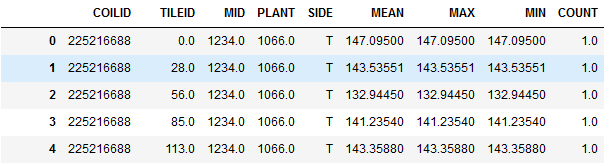
\includegraphics[width=0.9\textwidth]{img/eje2D.PNG}
     \caption{Ejemplo tabla GR\_QPValues}
     \label{f:tab2}
    \end{figure}
    \item  \textbf{V\_Coils:} contiene las bobinas (cuyas IDs se encuentran en el atributo SID) con la etiqueta colocada por parte del operario (atributo \emph{CLASSLABEL}). Además, tiene los valores mínimos y máximos de zinc (atributos \emph{ZnMin} y \emph{ZnMax}) que tiene que tener cada bobina. En total hay 1160 registros, o lo que es igual, 1160 bobinas clasificadas por parte de un operario. De dichas 1160 bobinas, 325 pertenecen a la clase NOK, lo que supondría un 28\% de los datos, mientras que 835 bobinas pertenecen a la clase OK, suponiendo un 72\% de los datos. Tras esta distribución, se puede ver cómo el conjunto de datos está desbalanceado. Finalmente, la Figura \ref{f:tab3} muestra un ejemplo de 5 registros correspondientes a esta tabla.
    \begin{figure}[h]
     \centering
      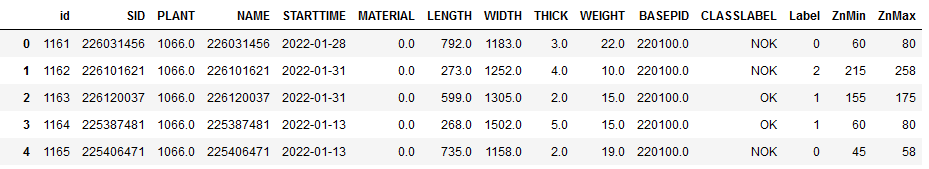
\includegraphics[width=1\textwidth]{img/ejeClas.PNG}
     \caption{Ejemplo tabla V\_Coilss}
     \label{f:tab3}
    \end{figure}
\end{itemize}

\subsubsection{Visualización de los datos}
En última instancia, en esta segunda fase se decidió realizar una pequeña visualización de los datos 1D de las bobinas proporcionadas junto con dos líneas verdes, representando los valores máximos y mínimos de zinc. Para ello, se llevó a cabo un desplegable con las IDs de las diferentes bobinas, de tal forma que al seleccionar una, se mostraban los gráficos de los cuatro sensores.

La Figura \ref{f:visu} muestra un ejemplo de visualización de las cuatro gráficas correspondientes a los diferentes sensores, junto con los diferentes valores de zinc medidos. En este caso se puede ver claramente, al observar el sensor 123, como la mayoría de las \emph{tejas} de la capa superior no cumplen con los requisitos de zinc. En cambio, si miramos los otros 3 sensores, se puede ver cómo la mayoría de las \emph{tejas} sí que cumple con los requisitos. 

\begin{figure}[h]
 \centering
  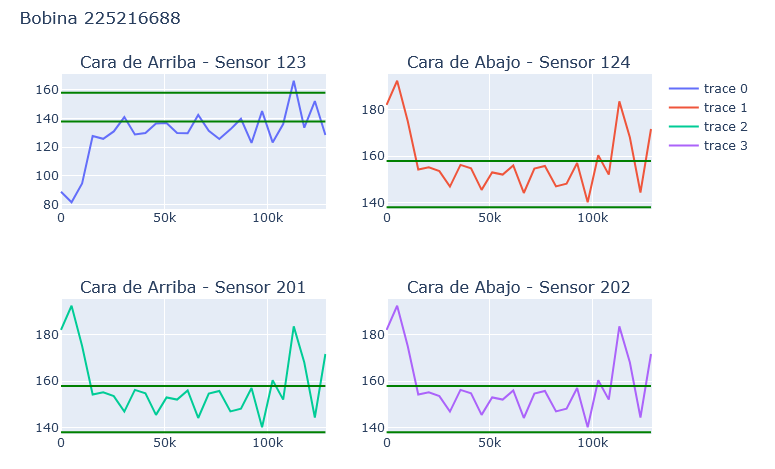
\includegraphics[width=0.9\textwidth]{img/visuaBobi.PNG}
 \caption{Ejemplo de Visualización para una Bobina}
 \label{f:visu}
\end{figure}

Este caso de ver como los valores medidos por el sensor 123 son bastante diferentes a los medidos 201 (ambos sensores miden la capa superior de la bobina), nos sorprendió, ya que los resultados deberían de ser similares al estar midiendo la misma capa, fue notificado a la empresa, aunque no se nos indicó nada al respecto.

\section{Preparación de los datos}
Esta tercera fase se ha dividido en dos grandes etapas: obtención de características y procesamiento de los datos para los modelos.

\subsubsection{Obtención de características}
Las características obtenidas para cada bobina fueron las indicadas por la empresa, ya que se estimaba que iban a ser las que mejores resultados iban a dar. 

Todas las características, que se van a mostrar a continuación, se han calculado para cada bobina y sensor y para los datos 1D y 2D. Es decir, para los datos 1D, se calcularon las características 4 veces, una para cada sensor. En cambio, para los datos 2D, al haber dos sensores, se calcularon dos veces.
\begin{itemize}
    \item \textbf{ZNMAX\_FAILURES:} se corresponde al número de tejas de la bobina que tiene una capa de zinc superior al estipulado. Los fallos se contarán desde que hay un fallo hasta que se encuentra una teja correcta, no un fallo por cada teja con un defecto.
    \item \textbf{ZNMIN\_FAILURES:} es el número de tejas de la bobina que tiene menos zinc del mínimo estipulado. Los fallos también se cuentan con el mismo criterio que el caso anterior.
    \item \textbf{CALIBRATED:} se corresponde al número de tejas en las que se ha producido un calibrado (reinico de los sensores).
    \item \textbf{TOTAL\_TILEID:} indica el número total de las tejas que tiene la bobina.
    \item \textbf{L\_DIS:} contiene el número de tejas que hay desde el inicio de la bobina hasta el último fallo antes de la mitad de la bobina.
    \item \textbf{R\_DIS:} indica el número de tejas que hay desde el fallo más cercano a la mitad y el final de la bobina.
\end{itemize}

Finalmente, dentro de las características calculadas para cada bobina, además de las anteriormente descritas, se calculó el mapa codificado de cada bobina. Este mapa consiste en que a cada teja de la bobina se le asigna uno de los siguientes valores:
\begin{itemize}
    \item \textbf{1:} en caso de que el valor de zinc medido en la teja sea mayor al estipulado.
    \item \textbf{0:} en caso de que el valor de zinc medido en la teja se encuentre entre el intervalo de zinc máximo y mínimo estipulado.
    \item \textbf{-1:} en caso de que el valor de zinc medido en la teja sea menor al estipulado.
\end{itemize}

Este mapa se almacenó en forma de \emph{array}, incluido para los datos 2D, ya que pese a que su mapa codificado es una matriz, por comodidad se ha guardado de esta forma. Será a la hora de leerlo cuando se transforme en matriz para poder utilizarlo correctamente.

La Figura \ref{f:fea1d} muestra un ejemplo de salida para los datos 1D. En ella se pueden ver todos los atributos anteriormente mencionados para cada sensor, incluido el mapa codificado correspondiente a la columna MAP. 

\begin{figure}[h]
 \centering
  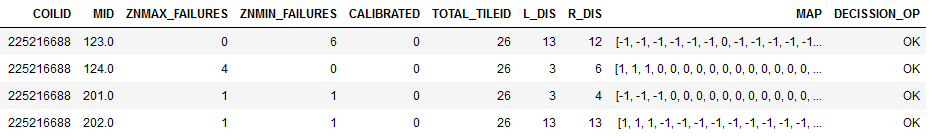
\includegraphics[width=1\textwidth]{img/fea1D.PNG}
 \caption{Ejemplo de características obtenidas para datos 1D}
 \label{f:fea1d}
\end{figure}

Por otro lado, la Figura \ref{f:fea2d} muestra un ejemplo para la misma bobina que la anterior pero con datos 2D. De igual manera, se pueden ver todas las características anteriormente descritas.

\begin{figure}[h]
 \centering
  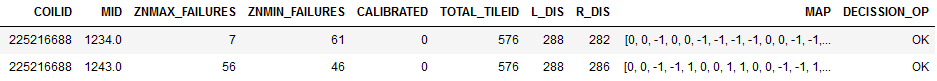
\includegraphics[width=1\textwidth]{img/fea2D.PNG}
 \caption{Ejemplo de características obtenidas para datos 2D}
 \label{f:fea2d}
\end{figure}

Para finalizar esta etapa, se guardaron las características obtenidas de los datos 1D y 2D en una base de datos. Para ello se crearon dos tablas, FEATURES\_1D y FEATURES\_2D, donde se almacena todo el contenido previamente calculado.

\subsubsection{Preparación de los datos para los modelos}
En esta segunda etapa de la tercera fase, era turno de preparar los datos obtenidos en la etapa anterior para que puedan ser utilizados por los modelos de \emph{TensorFlow}.

En primer lugar, se cargaron los mapas codificados de las bobinas 1D, y se decidió unir en un único \emph{array} cada par de sensores, es decir, unir los mapas de los sensores 123 y 124 y, por otro lado, los sensores 201 y 202.

El porqué de unirlos fue básicamente para tener los datos en una única dimensión, al igual que los originales, y así aplicar convoluciones de una dimensión. 

A continuación, sobre estos nuevos mapas unidos, se aplicó la técnica de \emph{padding}, que se basa en rellenar los datos con un valor para que todos ellos tengan las mismas dimensiones, ya que es necesario para las redes neuronales que se van a construir. En este caso, se rellenaron los datos con 0, hasta que todos los datos tuvieran una longitud de 208, puesto que fue el valor más grande encontrado dentro del conjunto de datos.

El porqué de añadir ceros se debe a que este valor representa que la teja es correcta, por tanto, si estamos añadiendo valores ficticios creíamos que era mejor añadir un valor correcto que no 1 o -1, indicando que la teja tiene algún defecto, y tal vez, afectando negativamente a la decisión del modelo.

En segundo lugar, se cargaron los mapas codificados de los datos 2D. Primero que todo, se reconstruyeron en forma de matriz, ya que como se ha comentado previamente, se guardaron en forma de \emph{array} por comodidad. Sobre estas matrices, también se aplicó la técnica de \emph{padding}, para que todos los mapas contaran con el mismo número de columnas.

Finalmente, con el resto de características, se decidió normalizar todos ellas, ya que de esta forma se contaba con valores para que los modelos trabajen. El tipo de normalización usada ha sido la conocida como normalización min-max, puesto que permite dejar los datos en valores comprendidos entre 0 y 1, y cuya fórmula es la siguiente:

$$DatoNorm = \frac{Dato - DatoMin}{{DatoMax} - {DatoMin}}$$

Ahora, ya se contaba con las características preparadas para ser usadas, pero antes había que transformar la clase de \emph{string} a \emph{int}. Dicha transformación fue: un 0 para la clase OK y un 1 para la clase NOK.

\section{Modelado}
En esta cuarta fase era turno de construir diversos modelos, con el fin de obtener el que mejor se adapte a este problema. 

En esta fase, se pueden distinguir dos etapas diferentes. Por un lado, se realizaron diversas pruebas con \emph{TensorFlow}, con el fin de generar diversos modelos y familiarizarse con su construcción. 

Por otro lado, tenemos la segunda etapa, en ella se construyeron los diferentes modelos con varios parámetros para buscar el mejor de todos.

\subsubsection{Pruebas}
En primer lugar, se crearon modelos individuales para familiarizarse con su construcción, la Figura \ref{f:modelo1}, muestra un ejemplo de ello.  

\begin{figure}[h]
 \centering
  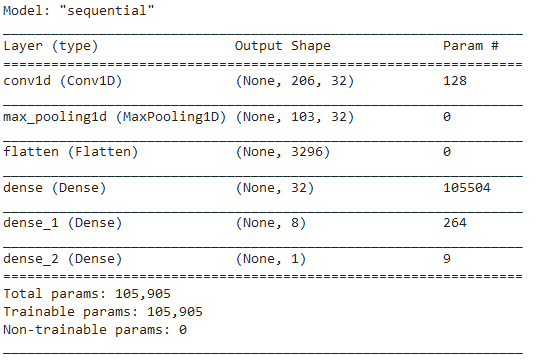
\includegraphics[width=0.8\textwidth]{img/modelo1.PNG}
 \caption{Ejemplo de Construcción de Modelo}
 \label{f:modelo1}
\end{figure}

Pese a empezar con modelos individuales, se usará la estrategia de validación cruzada de 5 \emph{folds}, ya que los resultados que se obtengan serán más robustos, al probar con diferentes conjuntos de valores para entrenar y validar los modelos.

Finalmente, en esta etapa también se decidió hacer pruebas utilizando alguna técnica para ajustar el conjunto de datos desbalanceado. En este caso se opta, debido al bajo número de registros, a realizar un sobremuestreo de los datos, y más concretamente aplicar la técnica SMOTE.

SMOTE (\emph{Synthetic Minority Oversampling Technique}) se basa en producir más ejemplos de la clase minoritaria de manera sintética. Para ello, busca dos ejemplos que estén próximos y genera uno nuevo con datos intermedios entre los dos ejemplos. Este proceso se repite varias veces hasta que el conjunto de datos se encuentra equilibrado.

Para concluir, indicar que los mejores resultados se consiguieron, aplicando validación cruzada, con datos a los que se les había aplicado el sobremuestreo, por lo que se decidirá usar en la siguiente etapa. Los resultados se pueden ver a continuación, en los que se muestran las matrices de confusión obtenidas para cada conjunto de datos. En las matrices, la primera fila se corresponde con la clase OK y la segunda fila con la clase NOK.

\begin{verbatim}
    -- Datos originales--
    La matriz de confusion obtenida es:
     [[ 44   6]
     [114  36]]

    -- Datos con sobremuestreo--
    La matriz de confusion obtenida es:
     [[40 10]
     [94 56]]
\end{verbatim}

Las precisiones obtenidas han sido de un 40\% y de un 48\% respectivamente, mostrándose unos mejores resultados en los datos con sobremuestreo.

\subsubsection{Construcción de modelos}
A la hora de construir los modelos finales, se han probado dos estrategias. Por un lado, crear modelos que utilicen tan solo los mapas codificados de las bobinas, y, por otro lado, crear modelos que utilicen todas las características previamente calculadas. Además, los modelos serán diferentes, como es obvio, según si emplean datos 1D o 2D. Todo ello aplicando la validación cruzada de 5 \emph{folds}.

Lo primero que se ha hecho en esta fase, ha sido separar una pequeña muestra de los datos originales: 150 registros de la clase NOK y 50 registros de la clase OK. De esta forma, se consigue que ningún modelo haya trabajado antes con estos datos y se puedan evaluar los modelos de una manera más exacta. Se ha separado esta muestra, ya que creemos que son datos suficientes como para evaluar y ver como se comportan los diferentes modelos. El resto de datos se usarán en la validación cruzada, de modo que en cada modelo algunos serán para entrenar y otros para validar.

En segundo lugar, se ha buscado el mejor criterio de discriminación para los modelos a construir. Para ello, se han probado un total de 5 valores diferentes y se ha obtenido el mejor de ellos, en función de las matrices de confusión y la precisión conseguida por cada criterio.

Los valores que se han probado han sido 0.3, 0.4, 0.5, 0.6, 0.7. Tras realizar diversas pruebas, se ha llegado a la conclusión que el mejor criterio es 0.3, tal y como se puede ver a continuación, donde se muestran las matrices de confusión y precisión obtenida (en las matrices de confusión la primera fila se corresponde a la clase Ok y la segunda a la clase NOK; con respecto a la precisión se corresponde a la tasa de acierto).

\begin{verbatim}
    Los resultados del criterio 0.3 son:

    La precisión obtenida ha sido 0.57
    La matriz de confusion obtenida es:
     [[33 17]
     [69 81]]
    
     Los resultados del criterio 0.4 son:
    
    La precisión obtenida ha sido 0.53
    La matriz de confusion obtenida es:
     [[36 14]
     [80 70]]
    
     Los resultados del criterio 0.5 son:
    
    La precisión obtenida ha sido 0.505
    La matriz de confusion obtenida es:
     [[40 10]
     [89 61]]
    
     Los resultados del criterio 0.6 son:
    
    La precisión obtenida ha sido 0.47
    La matriz de confusion obtenida es:
     [[40 10]
     [96 54]]
    
     Los resultados del criterio 0.7 son:
    
    La precisión obtenida ha sido 0.435
    La matriz de confusion obtenida es:
     [[ 42   8]
     [105  45]]
\end{verbatim}

Tras realizar estos dos pasos, ha sido turno de construir los modelos. Como ya se ha comentado previamente, se ha utilizado validación cruzada para generar 5 modelos en cada experimento. En todos estos modelos la estrategia utilizada ha sido la siguiente:
\begin{itemize}
    \item \textbf{Capa convolucional:} esta capa o capas, según las que se le indiquen, junto con el \emph{kernel} indicado y su activación tipo \emph{ReLU} (\emph{Rectified Linear Unit}), aplican la técnica de convolución a los datos de entrada.
    \item \textbf{Pooling:} aplica la técnica \emph{pooling} y devuelve el valor máximo.
    \item \textbf{Flatten:} transforma los datos de entrada en un vector unidimensional.
    \item \textbf{Dense:} capa o capas que contienen el número de neuronas indicado junto con una activación tipo \emph{ReLU}.
\end{itemize}

La activación ReLU, anteriormente mencionada, es una función que añade, entre otras mejoras, la no linealidad a la red neuronal al transformar todos los números negativos en cero.

Además, a la hora de entrenar el modelo, se ha utilizado un \emph{checkpoint}, que permite guardar el mejor modelo que se va obteniendo en las diferentes épocas, indicadas en el momento de su construcción, e ir sobreescribiéndole según se encuentra uno mejor, para quedarse con el modelo que menor \emph{loss} tenga. La función \emph{loss} permite evaluar el error obtenido entre las predicciones y los valores reales, de forma que cuanto menor sea mejor serán los resultados.

El tipo de \emph{loss} empleado ha sido \emph{binary cross entropy}, ya que suele ser la utilizada en problemas de clasificación binaria, cómo es el caso.

Con respecto a las predicciones finales de cada conjunto de modelos, se han sumado las predicciones de los 5 modelos y dividido entre 5, es decir, se ha calculado la media de los 5 modelos. A continuación, el valor se ha transformado a una clase u otra en función del criterio de discriminación, que, como ya se ha comentado anteriormente, se ha utilizado 0.3.

Finalmente, el número total de experimentos realizados ha sido 28. Para los datos 1D se han llevado a cabo 14 de ellos, de los cuales 7 han sido utilizando como dato de entrada el mapa codificado y otros 7 con todas las características normalizadas obtenidas de las bobinas.

Para los datos 2D se han efectuado los otros 14 experimentos restantes, con la misma distribución que en los datos 1D.

Además, en los experimentos que utilicen todos las características normalizadas obtenidas de las bobinas, se ha probado a realizar, para cada experimento, tras obtener los 5 modelos, crear un \emph{random forest} que con las 5 predicciones y los datos normalizados pretenda predecir la clase con el fin de saber si muestra mejores resultados. En resumen, los pasos que se han seguido para construir los \emph{random forest} son los siguientes:
\begin{enumerate}
    \item Con los datos de entrenamiento y test se obtienen los modelos con la validación cruzada.
    \item Sobre los modelos obtenidos se hacen predicciones de los datos de entrenamiento y test.
    \item Se unen las características normalizadas y las 5 predicciones de los modelos.
    \item Se construye un \emph{random forest} con los datos unidos y la clase real de los datos.
    \item Se efectúan predicciones con los datos de la muestra y se comparan con los resultados obtenidos de emplear únicamente los 5 modelos, con el fin de identificar el que mejores resultados da.
\end{enumerate}

A continuación se recogen los resultados obtenidos en los experimentos tanto para los datos 1D como para los datos 2D. En todas las matrices de confusión que se van a mostrar, la primera fila se corresponde a la clase OK, mientras que la segunda fila se corresponde a la clase NOK. Además, las precisiones vienen dadas en decimal, las cuales se corresponden a la tasa de acierto. Finalmente, añadir que las siglas RF se corresponden a los resultados del \emph{random forest}.

También, aclarar que, en los resultados, se muestra tan solo la matriz de confusión obtenida al aplicar los 5 modelos obtenidos en cada experimento al aplicar validación cruzada, y no la matriz de confusión individual de cada modelo, ya que los resultados importantes son aquellos en los que se utilizan los 5 modelos.
\subsubsection{Resultados datos 1D}
Se han realizado un total de 7 experimentos para los datos 1D sobre el mapa codificado de la bobina. Los resultados han sido los siguientes:

\begin{itemize}
    \item \textbf{Experimento 1:} en este caso los parámetros utilizados han sido una capa convolucional con 32 filtros , el tamaño de \emph{kernel} es 3, 300 iteraciones, y tres capas densas de tamaños, respectivamente, 32, 8 y 1. Los resultados obtenidos son los siguientes:
    \begin{verbatim}
        La precisión obtenida ha sido 0.535        
    \end{verbatim}
    La matriz de confusión obtenida se puede ver en la Figura \ref{f:exp1}.
    \begin{figure}[h]
     \centering
      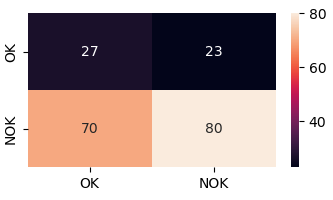
\includegraphics[width=0.5\textwidth]{img/exp1.PNG}
     \caption{Matriz de Confusión Experimento 1}
     \label{f:exp1}
    \end{figure}

    \item \textbf{Experimento 2:} en este segundo experimento se han empleado una capa convolucional con 64 filtros y con un \emph{kernel} de tamaño 5. Las iteraciones han sido 500, y las capas densas se han mantenido iguales que en el caso anterior. Los resultados son los siguientes:
    \begin{verbatim}
        La precisión obtenida ha sido 0.54
    \end{verbatim}
    La matriz de confusión obtenida se puede ver en la Figura \ref{f:exp2}.
    \begin{figure}[h]
     \centering
      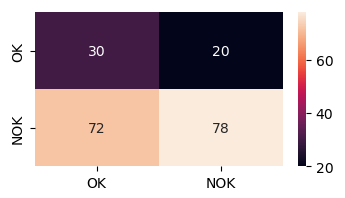
\includegraphics[width=0.5\textwidth]{img/exp2.PNG}
     \caption{Matriz de Confusión Experimento 2}
     \label{f:exp2}
    \end{figure}
    \item \textbf{Experimento 3:} en este tercer caso se ha usado una capa convolucional con 16 filtros y con un \emph{kernel} de tamaño 3. Las iteraciones han sido 300, y se han usado 5 capas densas de tamaños 64, 32, 16, 8 y 1. El resultado obtenido ha sido:
    \begin{verbatim}
        La precisión obtenida ha sido 0.54
    \end{verbatim}
    La matriz de confusión obtenida se puede ver en la Figura \ref{f:exp3}.
    \begin{figure}[h]
     \centering
      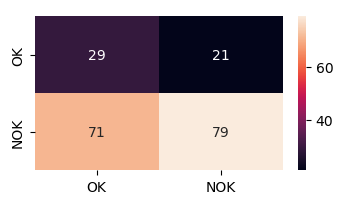
\includegraphics[width=0.5\textwidth]{img/exp3.PNG}
     \caption{Matriz de Confusión Experimento 3}
     \label{f:exp3}
    \end{figure}
    \item \textbf{Experimento 4:} en este cuarto caso se ha usado una capa convolucional de 16 filtros y con un \emph{kernel} de tamaño 5. Las iteraciones han sido 300 y se han empleado 3 capas densas de tamaño 32, 8 y 1.  Los resultados obtenidos han sido los siguientes:
    \begin{verbatim}
        La precisión obtenida ha sido 0.56
    \end{verbatim}
    La matriz de confusión obtenida se puede ver en la Figura \ref{f:exp4}.
    \begin{figure}[h]
     \centering
      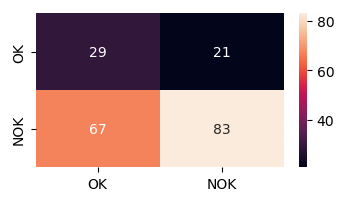
\includegraphics[width=0.5\textwidth]{img/exp4.PNG}
     \caption{Matriz de Confusión Experimento 4}
     \label{f:exp4}
    \end{figure}
    \item \textbf{Experimento 5:} en este quinto experimento se han usado 3 capas convolucionales con  16, 32 y 64 filtros y todas ellas con un \emph{kernel} de tamaño 3. Las iteraciones y las capas densas han sido las mimas que las del experimento anterior. Los resultados obtenidos han sido;
    \begin{verbatim}
        La precisión obtenida ha sido 0.57
    \end{verbatim}
    La matriz de confusión obtenida se puede ver en la Figura \ref{f:exp5}.
    \begin{figure}[h]
     \centering
      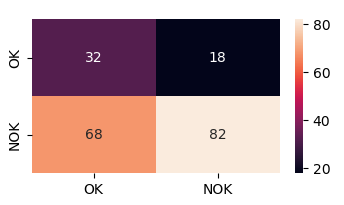
\includegraphics[width=0.5\textwidth]{img/exp5.PNG}
     \caption{Matriz de Confusión Experimento 5}
     \label{f:exp5}
    \end{figure}
    \item \textbf{Experimento 6:} en este penúltimo experimento se han mantenido los valores del experimento anterior pero aumentando las iteraciones a 500. Los resultados han sido:
    \begin{verbatim}
        La precisión obtenida ha sido 0.56
    \end{verbatim}
    La matriz de confusión obtenida se puede ver en la Figura \ref{f:exp6}.
    \begin{figure}[h]
     \centering
      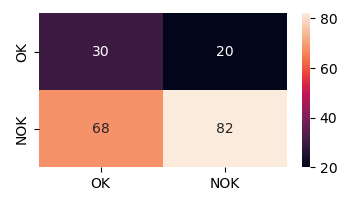
\includegraphics[width=0.5\textwidth]{img/exp6.PNG}
     \caption{Matriz de Confusión Experimento 6}
     \label{f:exp6}
    \end{figure}
    \item \textbf{Experimento 7:} en el último caso se han utilizado los mismos valores que en el experimento 5 pero cambiando el tamaño del \emph{kernel} a 5. Los resultados han sido:
    \begin{verbatim}
        La precisión obtenida ha sido 0.505
    \end{verbatim}
    La matriz de confusión obtenida se puede ver en la Figura \ref{f:exp7}.
    \begin{figure}[h]
     \centering
      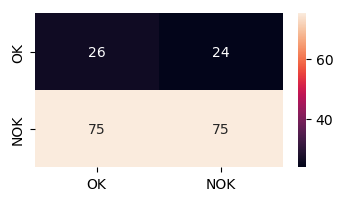
\includegraphics[width=0.5\textwidth]{img/exp7.PNG}
     \caption{Matriz de Confusión Experimento 7}
     \label{f:exp7}
    \end{figure}
\end{itemize}

Sobre el mapa codificado y los atributos normalizados se han realizado otros 7 experimentos, cuyos resultados son los siguientes (en los resultados se incluye la precisión utilizando únicamente el modelo y la precisión obtenida combinando los modelos con el \emph{Random Forest}):

\begin{itemize}
    \item \textbf{Experimento 8:} este primer experimento ha sido con una capa convolucional con 32 filtros y con un \emph{kernel} de tamaño 3. Además, ternía 300 iteraciones y 3 capas densas de tamaños 32, 8 y 1. Los resultados han sido:
    \begin{verbatim}
        La precisión obtenida ha sido 0.47
    \end{verbatim}
    La matriz de confusión obtenida se puede ver en la Figura \ref{f:exp8a}.
    \begin{verbatim}
        La precisión obtenida con el RF ha sido 0.475
    \end{verbatim}
    La matriz de confusión obtenida se puede ver en la Figura \ref{f:exp8b}.
    \begin{figure}[h]
     \centering
      \subfloat[Matriz Confusión 1]{
       \label{f:exp8a}
        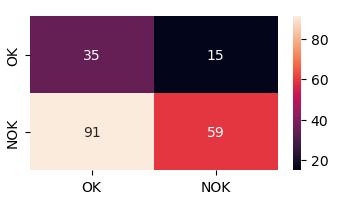
\includegraphics[width=0.3\textwidth]{img/exp8a.PNG}}
      \subfloat[Matriz Confusión 2]{
       \label{f:exp8b}
        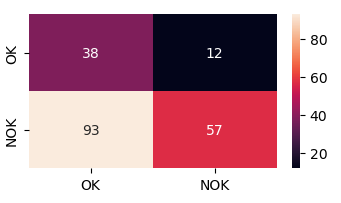
\includegraphics[width=0.3\textwidth]{img/exp8b.PNG}}  
     \caption{Matriz de Confusión Experimento 8}
     \label{f:exp8}
    \end{figure}
    \item \textbf{Experimento 9:} este segundo caso ha sido igual que el anterior pero con un \emph{kernel} de tamaño 5 y con 16 filtros. Los resultados se muestran a continuación:
    \begin{verbatim}
        La precisión obtenida ha sido 0.51
    \end{verbatim}
    La matriz de confusión obtenida se puede ver en la Figura \ref{f:exp9a}.
    \begin{verbatim}    
        La precisión obtenida con el RF ha sido 0.445
    \end{verbatim}
    La matriz de confusión obtenida se puede ver en la Figura \ref{f:exp9b}.
    \begin{figure}[h]
     \centering
      \subfloat[Matriz Confusión 1]{
       \label{f:exp9a}
        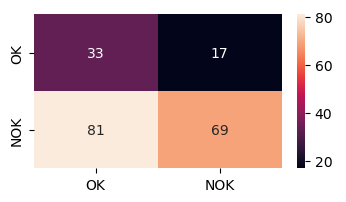
\includegraphics[width=0.3\textwidth]{img/exp9a.PNG}}
      \subfloat[Matriz Confusión 2]{
       \label{f:exp9b}
        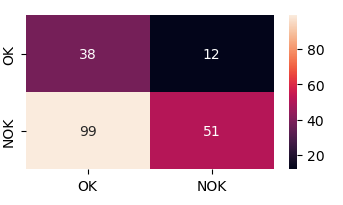
\includegraphics[width=0.3\textwidth]{img/exp9b.PNG}}  
     \caption{Matriz de Confusión Experimento 9}
     \label{f:exp9}
    \end{figure}
    
    \item \textbf{Experimento 10:} en este tercer experimento ha sido similar al anterior pero con 64 filtros. Los resultados han sido:
    \begin{verbatim}
        La precisión obtenida ha sido 0.485
    \end{verbatim}
    La matriz de confusión obtenida se puede ver en la Figura \ref{f:exp10a}.
    \begin{verbatim}
        La precisión obtenida con el RF ha sido 0.46
    \end{verbatim}
    La matriz de confusión obtenida se puede ver en la Figura \ref{f:exp10b}.
    \begin{figure}[h]
     \centering
      \subfloat[Matriz Confusión 1]{
       \label{f:exp10a}
        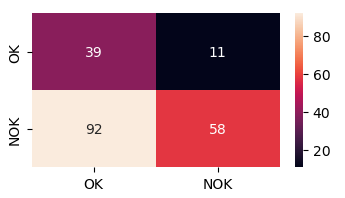
\includegraphics[width=0.3\textwidth]{img/exp10a.PNG}}
      \subfloat[Matriz Confusión 2]{
       \label{f:exp10b}
        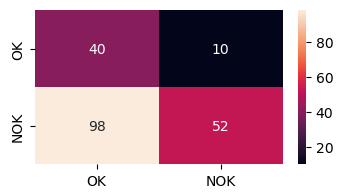
\includegraphics[width=0.3\textwidth]{img/exp10b.PNG}}  
     \caption{Matriz de Confusión Experimento 10}
     \label{f:exp10}
    \end{figure}
    
    \item \textbf{Experimento 11:} este cuarto caso ha sido igual que el primero pero con 16 filtros. Los resultados son:
    \begin{verbatim}
        La precisión obtenida ha sido 0.525
    \end{verbatim}
    La matriz de confusión obtenida se puede ver en la Figura \ref{f:exp11a}.
    \begin{verbatim}
        La precisión obtenida con el RF ha sido 0.47
    \end{verbatim}
    La matriz de confusión obtenida se puede ver en la Figura \ref{f:exp11b}.
    \begin{figure}[h]
     \centering
      \subfloat[Matriz Confusión 1]{
       \label{f:exp11a}
        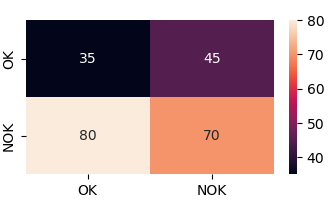
\includegraphics[width=0.3\textwidth]{img/exp11a.PNG}}
      \subfloat[Matriz Confusión 2]{
       \label{f:exp11b}
        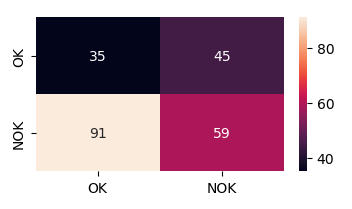
\includegraphics[width=0.3\textwidth]{img/exp11b.PNG}}  
     \caption{Matriz de Confusión Experimento 11}
     \label{f:exp11}
    \end{figure}
    
    \item \textbf{Experimento 12:} este quinto experimento ha sido igual que el anterior, solo que con 5 capas densas y de tamaños 64, 32, 16, 8 y 1. Se han obtenido los siguientes resultados:
    \begin{verbatim}
        La precisión obtenida ha sido 0.475
    \end{verbatim}
    La matriz de confusión obtenida se puede ver en la Figura \ref{f:exp12a}.
    \begin{verbatim}
        La precisión obtenida con el RF ha sido 0.455
    \end{verbatim}
    La matriz de confusión obtenida se puede ver en la Figura \ref{f:exp12b}.
    \begin{figure}[h]
     \centering
      \subfloat[Matriz Confusión 1]{
       \label{f:exp12a}
        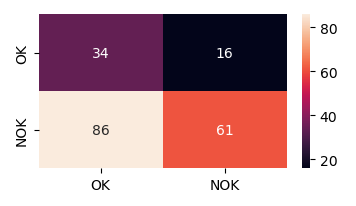
\includegraphics[width=0.3\textwidth]{img/exp12a.PNG}}
      \subfloat[Matriz Confusión 2]{
       \label{f:exp12b}
        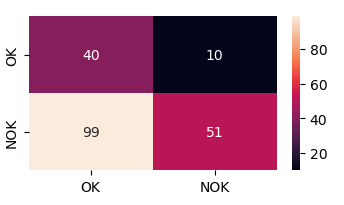
\includegraphics[width=0.3\textwidth]{img/exp12b.PNG}}  
     \caption{Matriz de Confusión Experimento 12}
     \label{f:exp12}
    \end{figure}
    
    \item \textbf{Experimento 13:} este penúltimo experimento ha sido igual que el anterior, pero con dos capas convolucionales con 32 y 64 filtros. Los resultados son:
    \begin{verbatim}
        La precisión obtenida ha sido 0.48
    \end{verbatim}
    La matriz de confusión obtenida se puede ver en la Figura \ref{f:exp13a}.
    \begin{verbatim}
        La precisión obtenida con el RF ha sido 0.455
    \end{verbatim}
    La matriz de confusión obtenida se puede ver en la Figura \ref{f:exp13b}.
    \begin{figure}[h]
     \centering
      \subfloat[Matriz Confusión 1]{
       \label{f:exp13a}
        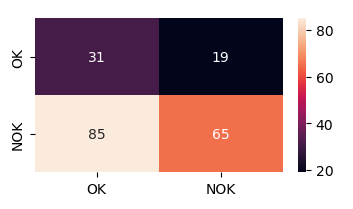
\includegraphics[width=0.3\textwidth]{img/exp13a.PNG}}
      \subfloat[Matriz Confusión 2]{
       \label{f:exp13b}
        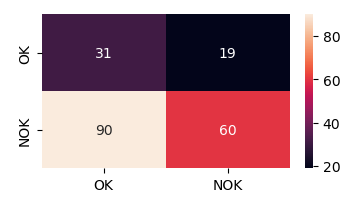
\includegraphics[width=0.3\textwidth]{img/exp13b.PNG}}  
     \caption{Matriz de Confusión Experimento 13}
     \label{f:exp13}
    \end{figure}
    \newpage
    \item \textbf{Experimento 14:} en el último caso, muy parecido al anterior, solo que con un \emph{kernel} de tamaño 5, se han obtenido los siguientes resultados:
    \begin{verbatim}
        La precisión obtenida ha sido 0.425
    \end{verbatim}
    La matriz de confusión obtenida se puede ver en la Figura \ref{f:exp14a}.
    \begin{verbatim}
        La precisión obtenida con el RF ha sido 0.435
    \end{verbatim}
    La matriz de confusión obtenida se puede ver en la Figura \ref{f:exp14b}.
    \begin{figure}[h]
     \centering
      \subfloat[Matriz Confusión 1]{
       \label{f:exp14a}
        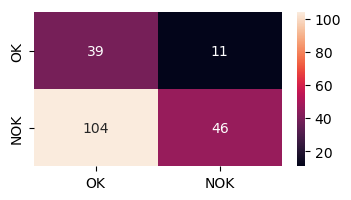
\includegraphics[width=0.3\textwidth]{img/exp14a.PNG}}
      \subfloat[Matriz Confusión 2]{
       \label{f:exp14b}
        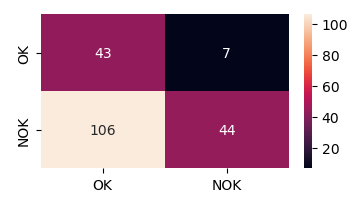
\includegraphics[width=0.3\textwidth]{img/exp14b.PNG}}  
     \caption{Matriz de Confusión Experimento 14}
     \label{f:exp14}
    \end{figure}    
\end{itemize}

\subsubsection{Resultados datos 2D}
Con respecto a los datos 2D, también se han realizado 7 experimentos sobre los mapas codificados de las bobinas. A continuación se muestran los resultados:

\begin{itemize}
    \item \textbf{Experimento 15:} en este primer caso se utiliza una capa convolucional con 32 filtros y un \emph{kernel} de tamaño 3x3. Además, se efectúan 100 iteraciones y tres capas densas de tamaños 32, 8 y 1. Los resultados han sido los siguientes:
    \begin{verbatim}
        La precisión obtenida ha sido 0.485
    \end{verbatim}
    La matriz de confusión obtenida se puede ver en la Figura \ref{f:exp15}.
    \begin{figure}[h]
     \centering
      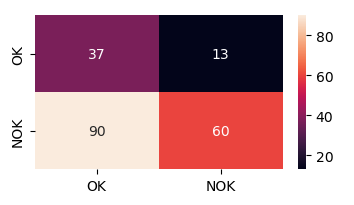
\includegraphics[width=0.5\textwidth]{img/exp15.PNG}
     \caption{Matriz de Confusión Experimento 15}
     \label{f:exp15}
    \end{figure}
    
    \item \textbf{Experimento 16:} este experimento es muy similar al anterior, solo que con 16 filtros. Los resultados son los siguientes:
    \begin{verbatim}
        La precisión obtenida ha sido 0.49
    \end{verbatim}
    La matriz de confusión obtenida se puede ver en la Figura \ref{f:exp16}.
    \begin{figure}[h]
     \centering
      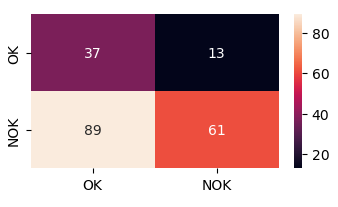
\includegraphics[width=0.5\textwidth]{img/exp16.PNG}
     \caption{Matriz de Confusión Experimento 16}
     \label{f:exp16}
    \end{figure}
    
    \item \textbf{Experimento 17:} este tercer caso es muy similar al primero, pero ahora el tamaño del \emph{kernel} es de 5x5. Sus resultados han sido:
    \begin{verbatim}
        La precisión obtenida ha sido 0.525
    \end{verbatim}
    La matriz de confusión obtenida se puede ver en la Figura \ref{f:exp17}.
    \begin{figure}[h]
     \centering
      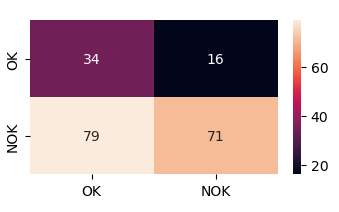
\includegraphics[width=0.5\textwidth]{img/exp17.PNG}
     \caption{Matriz de Confusión Experimento 17}
     \label{f:exp17}
    \end{figure}
    
    \item \textbf{Experimento 18:} este tercer experimento es similar al primero, pero con 64 filtros. Además, tiene 5 capas densas de tamaños 64, 32, 16, 8 y 1. Sus resultados han sido:
    \begin{verbatim}
        La precisión obtenida ha sido 0.53
    \end{verbatim}
    La matriz de confusión obtenida se puede ver en la Figura \ref{f:exp18}.
    \begin{figure}[h]
     \centering
      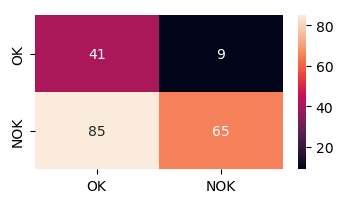
\includegraphics[width=0.5\textwidth]{img/exp18.PNG}
     \caption{Matriz de Confusión Experimento 18}
     \label{f:exp18}
    \end{figure}
    
    \item \textbf{Experimento 19:} este experimento ha sido similar al primero, solo que con 16 filtros y un \emph{kernel} de tamaño 5x5. Los resultados han sido:
    \begin{verbatim}
        La precisión obtenida ha sido 0.495
    \end{verbatim}
    La matriz de confusión obtenida se puede ver en la Figura \ref{f:exp19}.
    \begin{figure}[h]
     \centering
      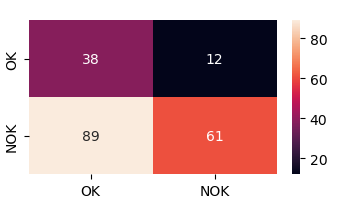
\includegraphics[width=0.5\textwidth]{img/exp19.PNG}
     \caption{Matriz de Confusión Experimento 19}
     \label{f:exp19}
    \end{figure}
    
    \item \textbf{Experimento 20:} este caso ha sido similar al primero pero con dos capas convolucionales con 16 y 32 filtros. Sus resultados han sido:
    \begin{verbatim}
        La precisión obtenida ha sido 0.49
    \end{verbatim}
    La matriz de confusión obtenida se puede ver en la Figura \ref{f:exp20}.
    \begin{figure}[h]
     \centering
      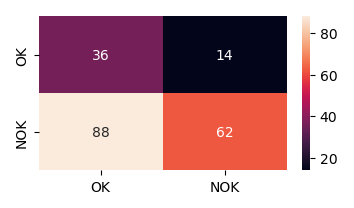
\includegraphics[width=0.5\textwidth]{img/exp20.PNG}
     \caption{Matriz de Confusión Experimento 20}
     \label{f:exp20}
    \end{figure}
    
    \item \textbf{Experimento 21:} este experimento ha sido similar al anterior, pero en este caso con tres capas convolucionales, de tamaños 16, 32 y 64. Los resultados han sido:
    \begin{verbatim}
        La precisión obtenida ha sido 0.54
    \end{verbatim}
    La matriz de confusión obtenida se puede ver en la Figura \ref{f:exp21}.
    \begin{figure}[h]
     \centering
      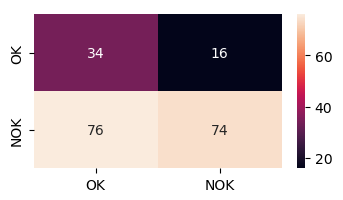
\includegraphics[width=0.5\textwidth]{img/exp21.PNG}
     \caption{Matriz de Confusión Experimento 21}
     \label{f:exp21}
    \end{figure}
    
\end{itemize}

Para los datos 2D juntando el mapa con los demás atributos, se han realizado de igual manera 7 experimentos. Además, al igual que para los datos 1D, se han añadido los resultados de usar \emph{Random Forest}. Todos los resultados se pueden ver a continuación:
\begin{itemize}
    \item \textbf{Experimento 22:} en este primer experimento se utiliza una capa convolucional con 32 filtros y un \emph{kernel} de 3x3. Además, se han empleado 100 iteraciones y 3 capas densas de tamaño 32, 8 y 1. Sus resultados han sido: 
    \begin{verbatim}
        La precisión obtenida ha sido 0.51
    \end{verbatim}
    La matriz de confusión obtenida se puede ver en la Figura \ref{f:exp22a}.
    \begin{verbatim}
        La precisión obtenida con el RF ha sido 0.5
    \end{verbatim}
    La matriz de confusión obtenida se puede ver en la Figura \ref{f:exp22b}.
    \begin{figure}[h]
     \centering
      \subfloat[Matriz Confusión 1]{
       \label{f:exp22a}
        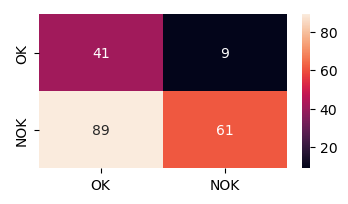
\includegraphics[width=0.3\textwidth]{img/exp22a.PNG}}
      \subfloat[Matriz Confusión 2]{
       \label{f:exp22b}
        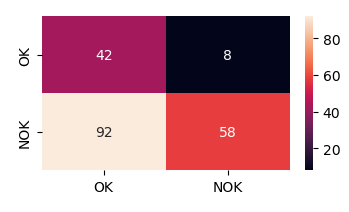
\includegraphics[width=0.3\textwidth]{img/exp22b.PNG}}  
     \caption{Matriz de Confusión Experimento 22}
     \label{f:exp22}
    \end{figure}    
    
    \item \textbf{Experimento 23:} este segundo experimento ha sido similar al anterior, pero con 16 filtros y el \emph{kernel} de tamaño 5x5. Los resultados han sido:
    \begin{verbatim}
        La precisión obtenida ha sido 0.505
    \end{verbatim}
    La matriz de confusión obtenida se puede ver en la Figura \ref{f:exp23a}.
    \begin{verbatim}        
        La precisión obtenida con el RF ha sido 0.53
    \end{verbatim}
    La matriz de confusión obtenida se puede ver en la Figura \ref{f:exp23b}.
    \begin{figure}[h]
     \centering
      \subfloat[Matriz Confusión 1]{
       \label{f:exp23a}
        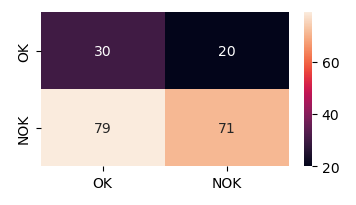
\includegraphics[width=0.3\textwidth]{img/exp23a.PNG}}
      \subfloat[Matriz Confusión 2]{
       \label{f:exp23b}
        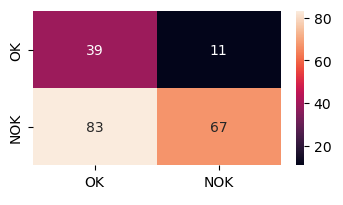
\includegraphics[width=0.3\textwidth]{img/exp23b.PNG}}  
     \caption{Matriz de Confusión Experimento 23}
     \label{f:exp23}
    \end{figure}    
    
    \item \textbf{Experimento 24:} este caso ha sido muy similar al primero pero con un \emph{kernel} de 5x5. Los resultados han sido:
    \begin{verbatim}
        La precisión obtenida ha sido 0.525
    \end{verbatim}
    La matriz de confusión obtenida se puede ver en la Figura \ref{f:exp24a}.
    \begin{verbatim}        
        La precisión obtenida con el RF ha sido 0.51
    \end{verbatim}
    La matriz de confusión obtenida se puede ver en la Figura \ref{f:exp24b}.
    \begin{figure}[h]
     \centering
      \subfloat[Matriz Confusión 1]{
       \label{f:exp24a}
        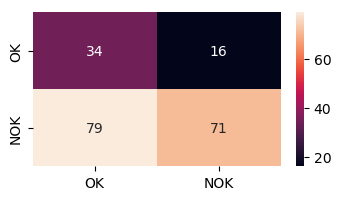
\includegraphics[width=0.3\textwidth]{img/exp24a.PNG}}
      \subfloat[Matriz Confusión 2]{
       \label{f:exp24b}
        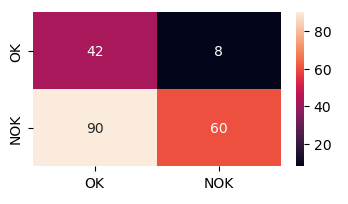
\includegraphics[width=0.3\textwidth]{img/exp24b.PNG}}  
     \caption{Matriz de Confusión Experimento 24}
     \label{f:exp24}
    \end{figure}    
    
    \item \textbf{Experimento 25:} este experimento ha sido como el primero, pero esta vez utilizando 16 filtros. Sus resultados han sido:
    \begin{verbatim}
        La precisión obtenida ha sido 0.49
    \end{verbatim}
    La matriz de confusión obtenida se puede ver en la Figura \ref{f:exp25a}.
    \begin{verbatim}
        La precisión obtenida con el RF ha sido 0.47
    \end{verbatim}
    La matriz de confusión obtenida se puede ver en la Figura \ref{f:exp25b}.
    \begin{figure}[h]
     \centering
      \subfloat[Matriz Confusión 1]{
       \label{f:exp25a}
        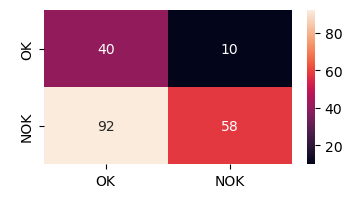
\includegraphics[width=0.3\textwidth]{img/exp25a.PNG}}
      \subfloat[Matriz Confusión 2]{
       \label{f:exp25b}
        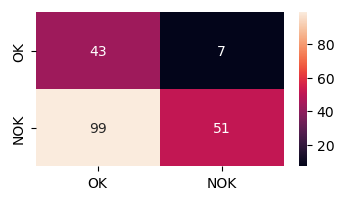
\includegraphics[width=0.3\textwidth]{img/exp25b.PNG}}  
     \caption{Matriz de Confusión Experimento 25}
     \label{f:exp25}
    \end{figure}    
    
    \item \textbf{Experimento 26:} este experimento ha sido similar al primero, pero las capas densas pasan a ser 5 y sus tamaños son 64, 32, 16, 8 y 1. Sus resultados son:
    \begin{verbatim}
        La precisión obtenida ha sido 0.515
    \end{verbatim}
    La matriz de confusión obtenida se puede ver en la Figura \ref{f:exp26a}.
    \begin{verbatim}
        La precisión obtenida con el RF ha sido 0.495
    \end{verbatim}
    La matriz de confusión obtenida se puede ver en la Figura \ref{f:exp26b}.
    \begin{figure}[h]
     \centering
      \subfloat[Matriz Confusión 1]{
       \label{f:exp26a}
        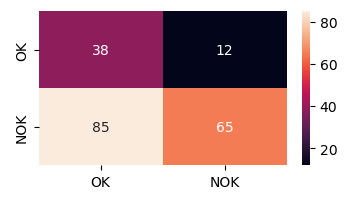
\includegraphics[width=0.3\textwidth]{img/exp26a.PNG}}
      \subfloat[Matriz Confusión 2]{
       \label{f:exp26b}
        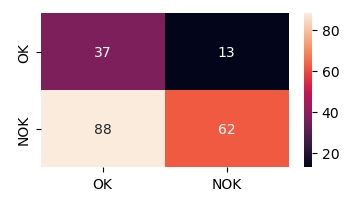
\includegraphics[width=0.3\textwidth]{img/exp26b.PNG}}  
     \caption{Matriz de Confusión Experimento 26}
     \label{f:exp26}
    \end{figure}    
    
    \item \textbf{Experimento 27:} en este sexto caso, similar al primero, se han añadido dos capas convolucionaales con 32 y 16 filtros. Los resultados son:
    \begin{verbatim}
        La precisión obtenida ha sido 0.51
    \end{verbatim}
    La matriz de confusión obtenida se puede ver en la Figura \ref{f:exp27a}.
    \begin{verbatim}
        La precisión obtenida con el RF ha sido 0.515
    \end{verbatim}
    La matriz de confusión obtenida se puede ver en la Figura \ref{f:exp27b}.
    \begin{verbatim}
    \end{verbatim}
    \begin{figure}[h]
     \centering
      \subfloat[Matriz Confusión 1]{
       \label{f:exp27a}
        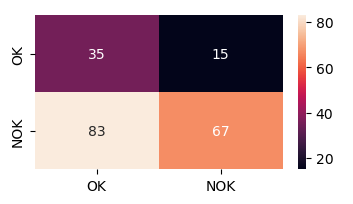
\includegraphics[width=0.3\textwidth]{img/exp27a.PNG}}
      \subfloat[Matriz Confusión 2]{
       \label{f:exp27b}
        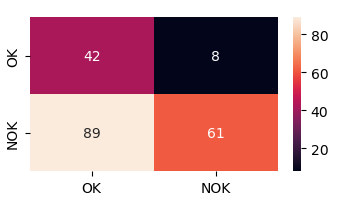
\includegraphics[width=0.3\textwidth]{img/exp27b.PNG}}  
     \caption{Matriz de Confusión Experimento 27}
     \label{f:exp27}
    \end{figure}    
    
    \item \textbf{Experimento 28:} este experimento ha sido similar al anterior, pero con una capa convolucional más. Sus tamaños son 16, 32 y 64, y cuyos resultados son:
    \begin{verbatim}
        La precisión obtenida ha sido 0.49
    \end{verbatim}
    La matriz de confusión obtenida se puede ver en la Figura \ref{f:exp28a}.
    \begin{verbatim}
        La precisión obtenida con el RF ha sido 0.475
    \end{verbatim}
    La matriz de confusión obtenida se puede ver en la Figura \ref{f:exp28b}.
    \begin{figure}[h]
     \centering
      \subfloat[Matriz Confusión 1]{
       \label{f:exp28a}
        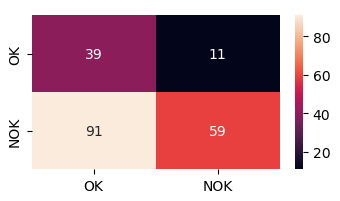
\includegraphics[width=0.3\textwidth]{img/exp28a.PNG}}
      \subfloat[Matriz Confusión 2]{
       \label{f:exp28b}
        \includegraphics[width=0.3\textwidth]{img/exp28b.PNG}}  
     \caption{Matriz de Confusión Experimento 28}
     \label{f:exp28}
    \end{figure}    
    
\end{itemize}

\section{Evaluación}
En esta quinta y penúltima fase, se han analizado los resultados obtenidos en los 28 experimentos realizados en la fase anterior.  

Lo primero que resalta son los malos resultados, ya que ninguno de los 28 experimentos han mostrado una buena precisión, de hecho, casi todos están con una precisión de entre el 50\% y 60\%.

Si comparamos los resultados entre los datos 1D y 2D, se ve como las precisiones más altas son las del primer tipo de datos, algo que puede resultar extraño, ya que se puede presuponer que los datos 2D mostrarán algún patrón o característica que haga que el modelo sea mejor, pero no ha sido el caso. Es por ello, que se cree que esto se debe a que en los datos proporcionados, el operario usa para clasificar las bobinas los datos 1D, de ahí esos posibles mejores resultados.

Si comparamos los resultados obtenidos directamente con los modelos a los obtenidos por el \emph{random forest}, se ve como este último, casi siempre es similar o un poco peor que si utilizamos solo los modelos.

Finalmente, el mejor resultado, se ha obtenido con el experimento 5 de los datos 1D empleando tan solo el mapa codificado de la bobina, por lo que será este el que se empleará en la siguiente fase. 

\section{Despliegue}
En esta sexta y última fase, ha sido turno de construir la aplicación final del proyecto, sobre la cual se puedan cargar datos de bobinas medidos por sensores y predecir y si serán bobinas válidas o no. 

La construcción de la aplicación se ha basado en dos partes. Por un lado, tenemos un \emph{notebook} donde se podrá elegir la base de datos donde se encuentran los datos y visualizar los resultados. Y, por otro lado, tenemos un archivo de \emph{Python} que contiene las diferentes funciones y que encapsula, de cara al usuario, todo el proceso, con el fin de dejar la aplicación lo vas sencilla y visual posible. 

Con respecto a los modelos usados para las predicciones, se han correspondido a los del experimento 5 sobre los datos 1D, ya que, como ya se ha visto en la fase anterior, han sido los que mejores resultados han dado. 

Además, para añadirle más funcionalidad a la aplicación, cada vez que se realizan predicciones sobre un modelo, se genera un archivo CSV que contiene todas las características obtenidas de la bobina, puesto que puede ser interesante almacenar los valores por si fuesen de utilidad al operario. También, se ha creado un histórico donde se almacenan las predicciones de las bobinas para poder consultarlas en el futuro sin la necesidad de tener que volver a cargar los datos.

El resultado se puede ver en la Figura \ref{f:apli1}, donde se aprecia la tabla con las diferentes características calculadas y el mapa codificado de la bobina. Además, más abajo se puede ver la predicción obtenida por los modelos según los datos obtenidos por cada par de sensores.

\begin{figure}[h]
 \centering
  \includegraphics[width=1\textwidth]{img/salidaAp.PNG}
 \caption{Ejemplo de Resultado de la Aplicación}
 \label{f:apli1}
\end{figure}

Y como se ha comentado, se ha generado a su vez un archivo CSV con todos los atributos calculados de la bobina y su mapa codificado para cada sensor. La Figura \ref{f:apli2}, muestra el CSV generado para la bobina de ejemplo mostrada en la imagen anterior. 

\begin{figure}[h]
 \centering
  \includegraphics[width=1\textwidth]{img/csv.PNG}
 \caption{Ejemplo de Resultado del CSV Genrado por la Aplicación}
 \label{f:apli2}
\end{figure}

Y también se ha generado un archivo historial.txt que contiene el registro de predicciones. La Figura \ref{f:apli3}, muestra dicho resultado. 

\begin{figure}[h]
 \centering
  \includegraphics[width=0.5\textwidth]{img/historial.PNG}
 \caption{Ejemplo de Resultado del histroial.txt Genrado por la Aplicación}
 \label{f:apli3}
\end{figure}

Además, si siguiéramos realizando predicciones, se generaría un CSV correspondiente a la bobina y en el fichero correspondiente al historial se añadirían al final la nueva información.